% This LaTeX was auto-generated from MATLAB code.
% To make changes, update the MATLAB code and export to LaTeX again.

\documentclass{article}

\usepackage[utf8]{inputenc}
\usepackage[T1]{fontenc}
\usepackage{lmodern}
\usepackage{graphicx}
\usepackage{color}
\usepackage{hyperref}
\usepackage{amsmath}
\usepackage{amsfonts}
\usepackage{epstopdf}
\usepackage[table]{xcolor}
\usepackage{matlab}

\sloppy
\epstopdfsetup{outdir=./}
\graphicspath{ {./PSASIM_images/} }

\begin{document}

\matlabtitle{Point Source Approximation For Simulating Extracellular Recording}

\begin{matlabcode}

% Written by Jesse Hurtado

% Simulation of two neurons firing in proximity to an electrode array. 
% This simulation includes two functions, PSA1 and PSA2, point source approximation 1 and 2.


% PSA1 will simulate an EXRTACELLULAR POTENTIAL RECORDING using a POINT
% SOURCE APPROXIMATION based on the Hodgkin-Huxley model, which assumes the current source acts as a point and
% the potential at a distance r away from the source can be approximated
% using a simple linear equation based on Koch, Buzaki, and Gold Point Source Approximation. 

% This PSA assumes the extracellular medium
% is homogeneous in conductivity. PSA takes three arguments, 1 = current
% amplitude (in pA) stimulating the distant neuron, 2 = distance from the
% recording electrode in microns, and 3 = noise that will cause variable
% spiking.

% PSA2 will simulate EXTRACELLULAR POTENTIAL RECORDING using a POINT SOURCE
% APPROXIMATION (PSA) based on the Connors Stevens model.

% Increasing the distance r (microns) from the electrode will, as proposed,
% decrease the recorded extracellular potential, and the amplitude of the
% overall trace changes as a a function of r. This can be demonstrated by
% varying the parameter r. 

% Using PSA, we can simulate extracellular
% recording, and sum their voltage traces to produce a simulated recording that models what a utah array recording electrode might detect.

% This simulation works best with a slight difference in applied currents
% as the frequency of spikes will be slighly out of phase and more individual spikes
% will appear in the summed trace.

% Finally, noise can be added to the trace to simulate LFP. Adding noise
% this way does not affect excitability of either neurons. 

% Each time the simulation is run, a unique trace will be produced.

% PSA can be adapted to other dynamic models
\end{matlabcode}


\begin{matlabcode}
% SIMULATE UTAH RECORDING OF TWO HH NEURONS 

% Time Vector 

dt=0.00002;           % time step (s)
tmax=1.1;             % max time value 1 second (s)
tvect= 0:dt:tmax;     % time vector, a second 

% LFP Noise Vector
hi = 16;             
LFP_vec = randn(1, length(tvect));
LFP_vec = LFP_vec*hi;


T1 = PSA1(5,7,0.0002);  % Simulate the PSA of a neuron with applied current of 5 nA, 7 microns away from recording electrode, with added noise to vary spiking.
\end{matlabcode}
\begin{center}
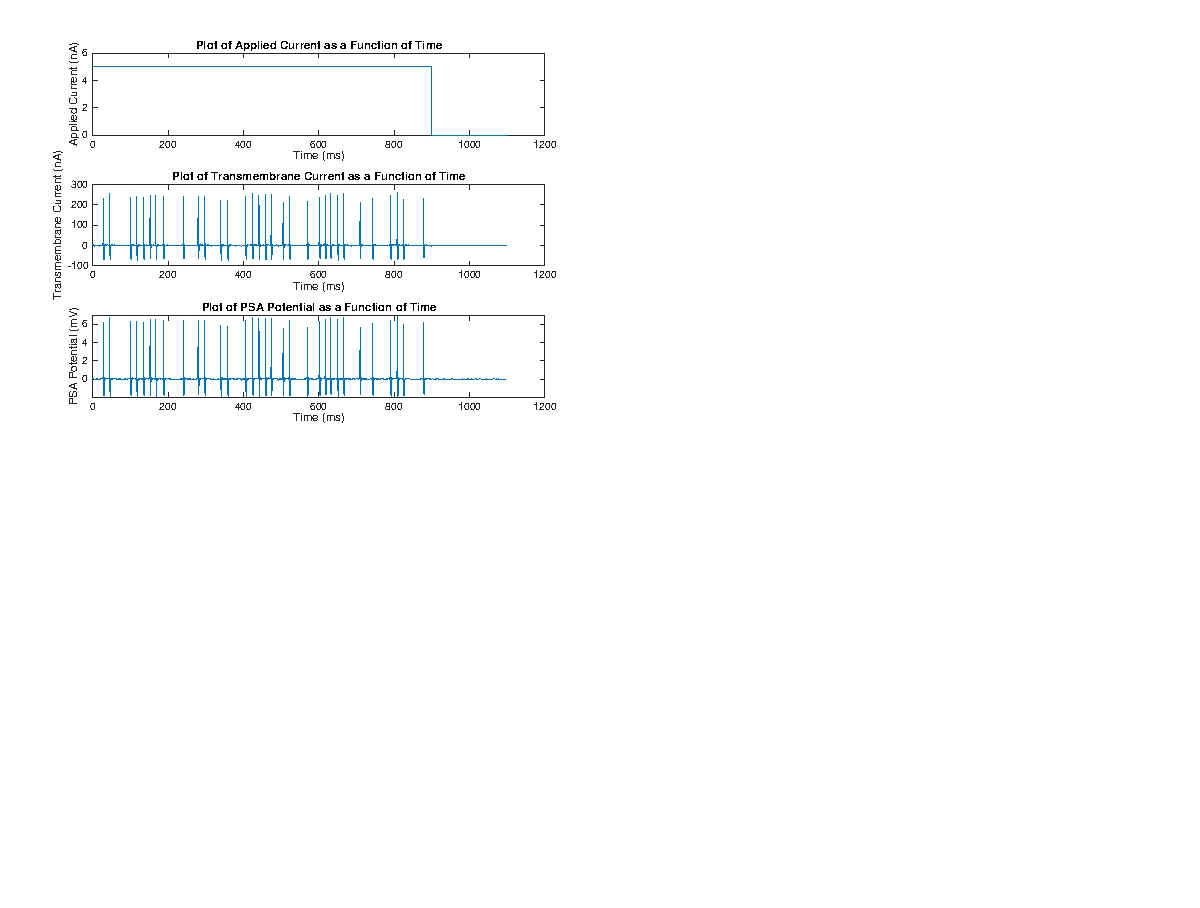
\includegraphics[width=\maxwidth{56.196688409433015em}]{figure_0.eps}
\end{center}
\begin{matlabcode}
T2 = PSA1(5,13,0.0002); % Simulate the PSA of a neuron with applied current of 5 nA, 13 microns away from recording electode, with added noise.
\end{matlabcode}
\begin{center}
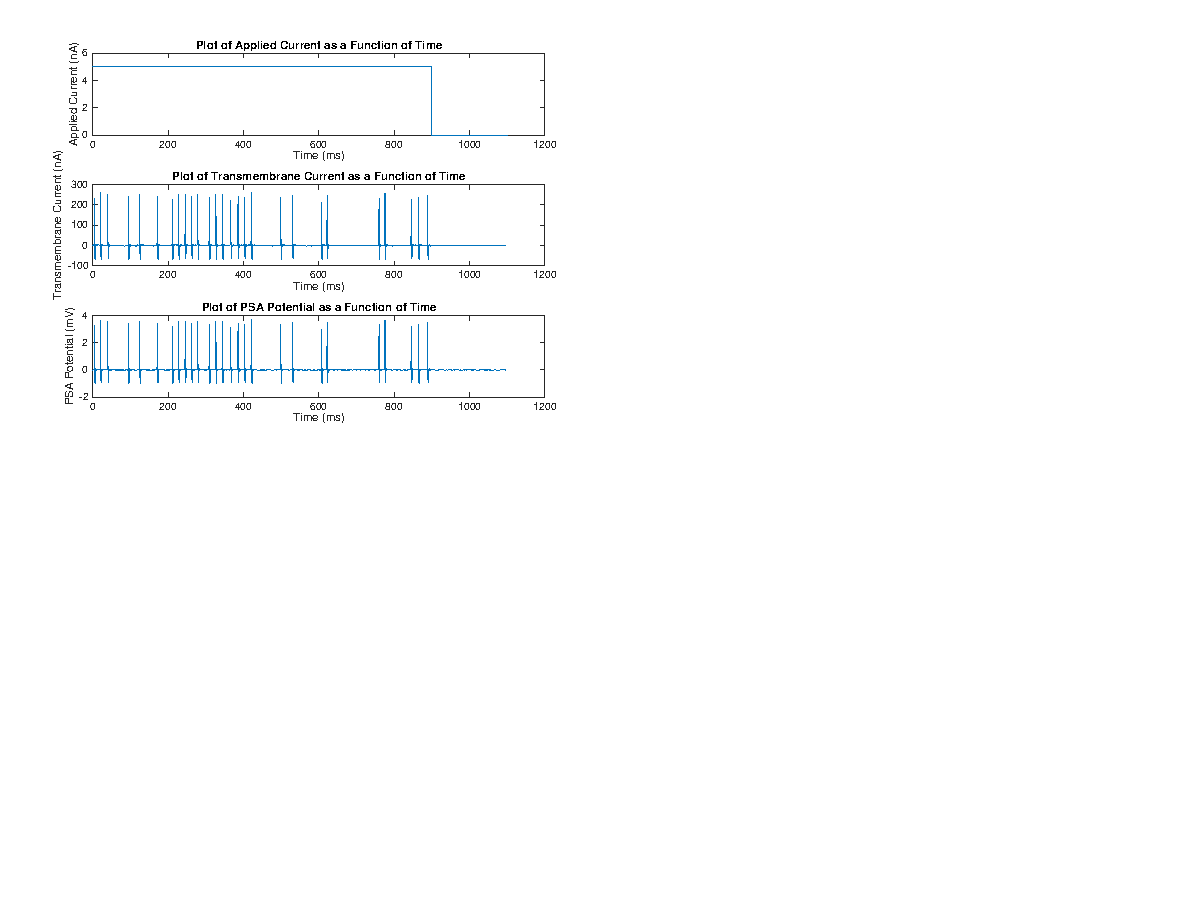
\includegraphics[width=\maxwidth{56.196688409433015em}]{figure_1.eps}
\end{center}
\begin{matlabcode}
T3 = T1+T2;             % Sum the voltage trace outputs

T3 = T3*100 + LFP_vec;  % Add LFP noise, final trace 

% This is done to remove artifacts present at the time of the start of the
% pulse

start_time = 0.1;  % Start time to remove (in seconds)
start_index = find(tvect >= start_time, 1);  % Find the index corresponding to the start time
T3 = T3(start_index:end);
tvect = tvect(start_index:end);              % Remove the time values before the start index
spikeTimes = detectSpikes(T3,tvect,200); % Detect spikes


%Plot 
figure;
plot(tvect,T3);
hold on
plot(spikeTimes, 200*ones(size(spikeTimes)), 'r.', 'MarkerSize', 15);
title('Simulation of Utah Array with Two HH neurons')  
xlabel('Time (ms)');
ylabel('Recorded Potential (uV)');
hold off
\end{matlabcode}
\begin{center}
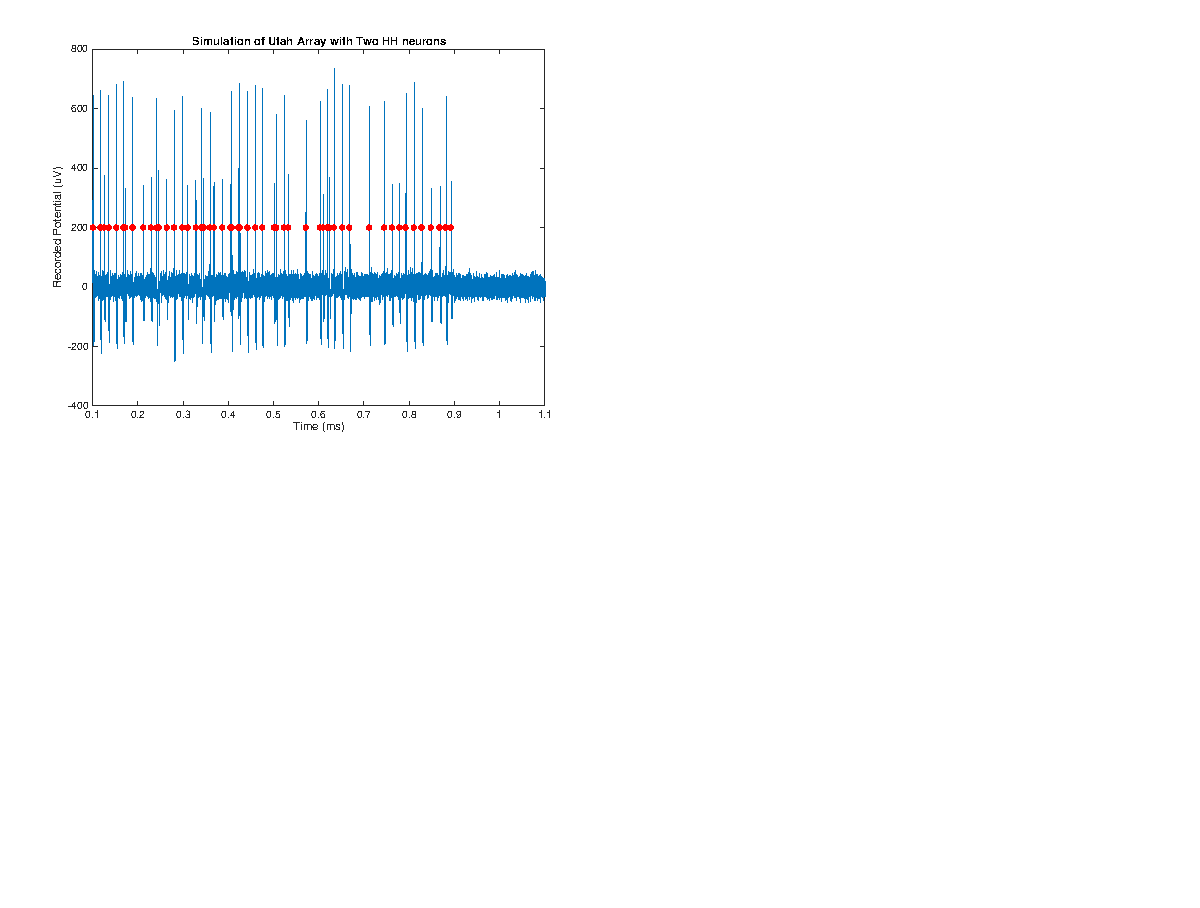
\includegraphics[width=\maxwidth{56.196688409433015em}]{figure_2.eps}
\end{center}


\begin{matlabcode}
% SIMULATE UTAH RECORDING OF TWO CONNORS STEVENS NEURONS 

clear

% Time Vector 

dt=0.00002;           % time step (s)
tmax=1.1;             % max time value 1 second (s)
tvect= 0:dt:tmax;     % time vector, a second 

% LFP Noise Vector
hi = 16;               % noise scalar       
LFP_vec = randn(1, length(tvect)); % empty LFP vector 
LFP_vec = LFP_vec*hi;  % scaled LFP vector 

V1 = PSA2(5,7,0.0002);   % run PSA2 (Connors Stevens) simulation for a neuron 7 microns away with a 5 nA applied current with noise.
\end{matlabcode}
\begin{center}
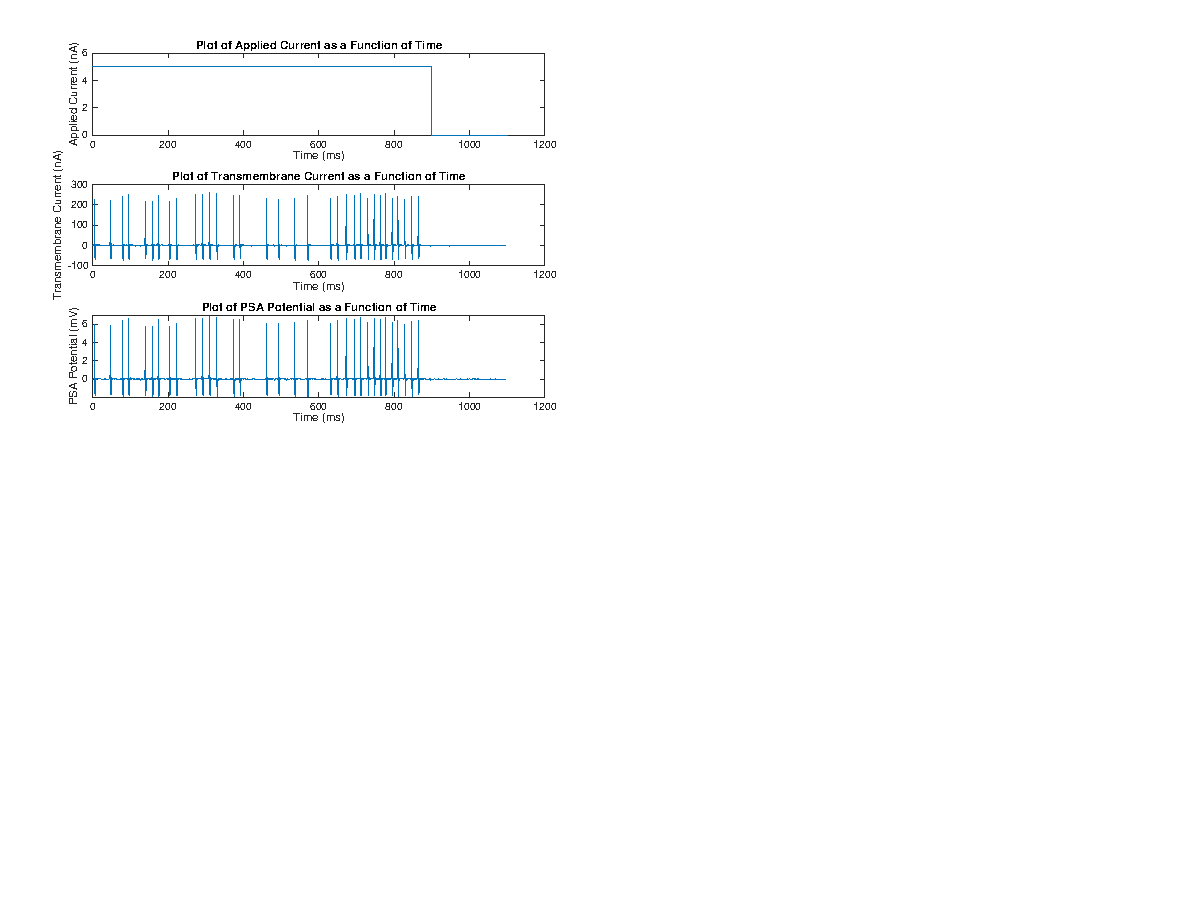
\includegraphics[width=\maxwidth{56.196688409433015em}]{figure_3.eps}
\end{center}
\begin{matlabcode}
V2 = PSA2(5,13,0.0002);  % run PSA2 (Connors Stevens) simulation for a neuron 15 microns away with a 5 nA applied current with noise.
\end{matlabcode}
\begin{center}
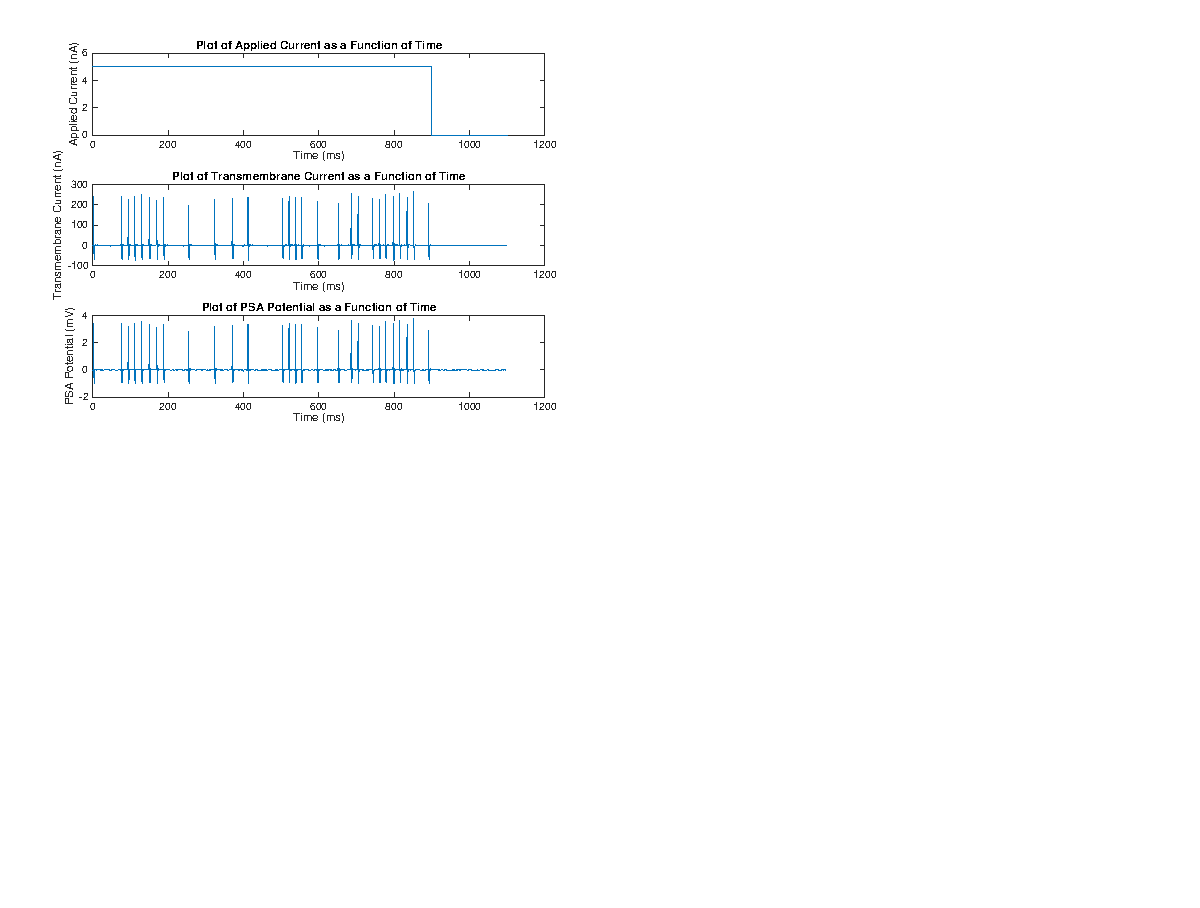
\includegraphics[width=\maxwidth{56.196688409433015em}]{figure_4.eps}
\end{center}
\begin{matlabcode}

V3 = V1+V2;                % Sum the voltage trace outputs

V3 = V3*100 + LFP_vec;     % Add LFP noise, final trace 

start_time = 0.1;  % Start time to remove (in seconds)
start_index = find(tvect >= start_time, 1);  % Find the index corresponding to the start time
V3 = V3(start_index:end);
tvect = tvect(start_index:end);  % Remove the time values before the start index

spikeTimes = detectSpikes(V3,tvect,200); % Detect spikes


%Plot
figure;
plot(tvect,V3);
hold on
plot(spikeTimes, 200*ones(size(spikeTimes)), 'r.', 'MarkerSize', 15);title('Simulation of Utah Array with Two Connors Stevens Neurons')  
xlabel('Time (ms)');
ylabel('Recorded Potential (uV)');
\end{matlabcode}
\begin{center}
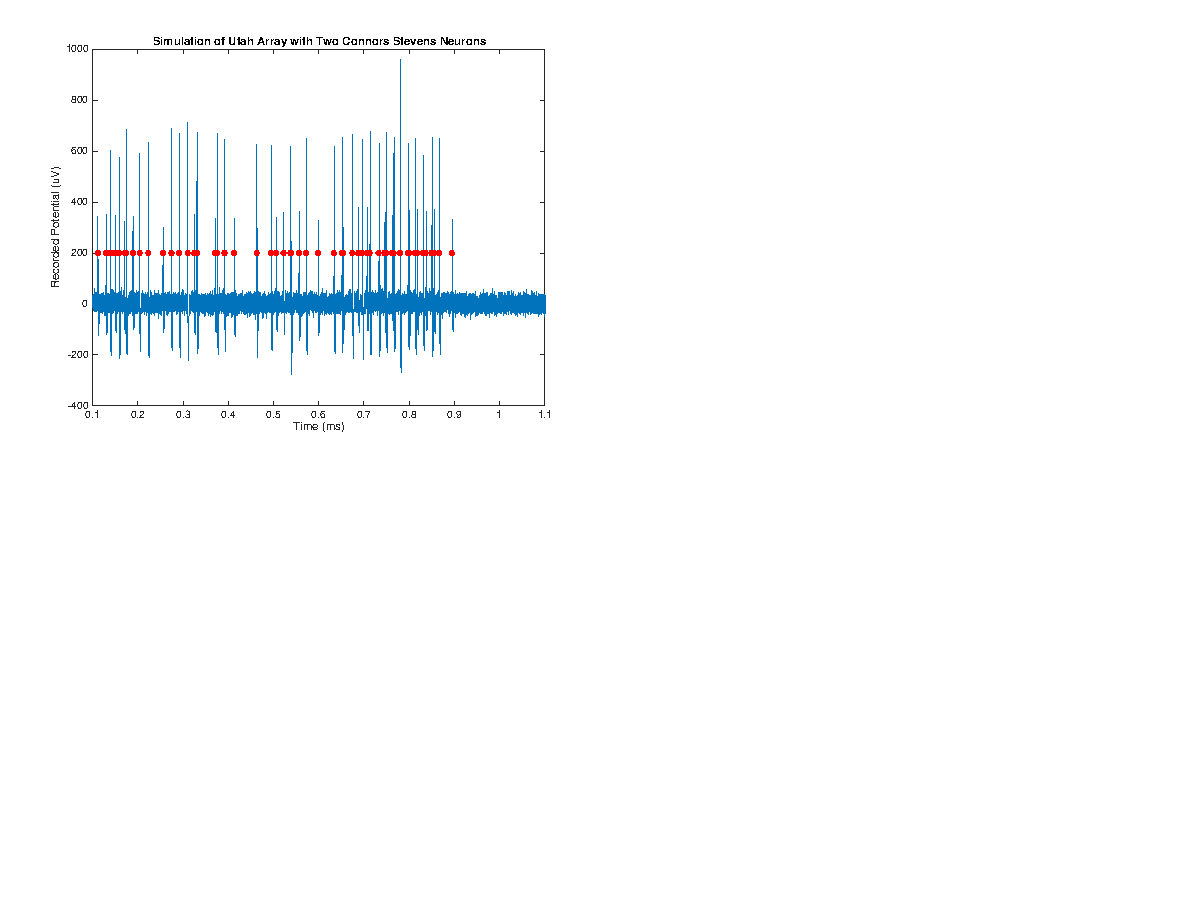
\includegraphics[width=\maxwidth{56.196688409433015em}]{figure_5.eps}
\end{center}
\begin{matlabcode}


\end{matlabcode}


\begin{matlabcode}
function [j] = PSA1(I,r,noise)
% Point Source Approximation based on HODGKIN-HUXLEY 
% inputs are I in nA and r (distance from recroding electode) in microns,

% HH Parameters 

Gmax_Na=12e-6;       % maximum sodium conductance (S)
Gmax_K=3.6e-6;       % maximum delayed rectifier conductance (S)
G_L=30e-9;           % leak conductance (S)
E_Na=45e-3;          % sodium reversal potential (V)
E_K=-82e-3;          % potassium reversal potential (V)
E_L=-60e-3;          % leak reversal potential (V)
Cm=100e-12;          % membrance capaictance (F)

% Point Source Approximation Values 

sigma = 0.43;        % Siemens / m^2 medium conductivity
R = r * 10^-7;       % in meters (one micron = 1e-6 meters)
q = noise;           % noise scalar


dt=0.00002;            % time step (s)
tmax=1.1;              % max time value (s)
tvect=0:dt:tmax;       % time vector (s)
Vm=zeros(size(tvect)); % membrane potential Vm vector
Vm(1)=-0.065;          % set initial condition (V)
m=zeros(size(tvect));  % gating variable m vector
m(1)=0.05;             % set initial condition
h=zeros(size(tvect));  % gating variable h vector
h(1)=0.5;              % set initial condition
n=zeros(size(tvect));  % gating variable n vector
n(1)=0.35;             % set initial condition

dVmdt = zeros(size(tvect));  % store value of dVdt for PSA
Im = zeros(size(tvect));     % empty vector for transmembrane current 
theta = zeros(size(tvect));  % point source approximation for EXTRACELLULAR POTENTIAL 


step_time=0.9;               % step duration (s)
start_time=0;                % start time of the step (s)
step_Iapp= I * 10^-10;       % applied current value (A)
Iapp_vect=zeros(size(tvect));% applied current vector (A)
step_indices = tvect >= start_time & tvect < (start_time + step_time); % find indices corresponding to step duration
Iapp_vect(step_indices)=step_Iapp; % set step current for the specified duration


for i=2:length(tvect)             % integrate over time
    dVmdt(i-1)=(1/Cm) * (G_L*(E_L-Vm(i-1)) + Gmax_Na*((m(i-1))^3)*h(i-1)*(E_Na-Vm(i-1)) + Gmax_K*((n(i-1))^4)*(E_K-Vm(i-1)) + Iapp_vect(i-1));   % define Vm rate of change
    Vm(i)=Vm(i-1)+dVmdt(i-1)*dt +randn()*noise;       % update Vm

    dmdt=(((10^5)*(-Vm(i-1)-0.045))/(exp(100*(-Vm(i-1)-0.045))-1))*(1-m(i-1)) - (4*(10^3)*exp((-Vm(i-1)-0.070)/0.018))*m(i-1);   % define m rate of change
    m(i)=m(i-1)+dmdt*dt;          % update m

    dhdt=(70*exp(50*(-Vm(i-1)-0.070)))*(1-h(i-1)) - ((10^3)/(1+exp(100*(-Vm(i-1)-0.040))))*h(i-1);   % define h rate of change
    h(i)=h(i-1)+dhdt*dt;          % update h

    dndt=(((10^4)*(-Vm(i-1)-0.060))/(exp(100*(-Vm(i-1)-0.060))-1))*(1-n(i-1)) - (125*exp((-Vm(i-1)-0.070)/0.08))*n(i-1);   % define n rate of change
    n(i)=n(i-1)+dndt*dt;          % update n

    Im(i-1) = dVmdt(i-1)*Cm;      % calculate Im 
    theta(i-1) = Im(i-1)/(4*pi*sigma*R); %calculate PSA potential 

end

% Plot
figure;
subplot(3,1,2);
plot(tvect*10^3,Im*10^10);
title('Plot of Transmembrane Current as a Function of Time')  
xlabel('Time (ms)');
ylabel('Transmembrane Current (nA)');

subplot(3,1,1);
plot(tvect*10^3,Iapp_vect*10^10);
title('Plot of Applied Current as a Function of Time')  
xlabel('Time (ms)');
ylabel('Applied Current (nA)');

subplot(3,1,3);
plot(tvect*10^3,theta*10^3);
title('Plot of PSA Potential as a Function of Time')  
xlabel('Time (ms)')
ylabel('PSA Potential (mV)')
j = theta*10^3;
end

function [V] = PSA2(I,r,noise)
% Point Source Approximation based on Connors Stevens Model
% inputs are I in nA and r (distance from recroding electode) in microns,
% and noise 

% Connors Stevens Parameters
Gmax_Na=12e-6;       % maximum sodium conductance (S)
Gmax_K=3.6e-6;       % maximum delayed rectifier conductance (S)
G_L=30e-9;           % leak conductance (S)
E_Na=45e-3;          % sodium reversal potential (V)
E_K=-82e-3;          % potassium reversal potential (V)
E_L=-60e-3;          % leak reversal potential (V)
Cm=100e-12;          % membrance capaictance (F)

Gmax_A=25e-9;          % A-current conductance (S)
E_A=-70e-3;            % A-current reversal potential (V)

% Initialize Vectors 
dt=0.00002;            % time step (s)
tmax=1.1;              % max time value (s)
tvect=0:dt:tmax;       % time vector (s)
Vm=zeros(size(tvect)); % membrane potential Vm vector
Vm(1)=-0.065;          % set initial condition (V)
m=zeros(size(tvect));  % gating variable m vector
m(1)=0.05;             % set initial condition
h=zeros(size(tvect));  % gating variable h vector
h(1)=0.5;              % set initial condition
n=zeros(size(tvect));  % gating variable n vector
n(1)=0.35;             % set initial condition
a=zeros(size(tvect));  % gating variable a vector
a(1)=0.05;             % set initial condition
b=zeros(size(tvect));  % gating variable b vector
b(1)=0.05;             % set initial condition

%PSA Values 
sigma = 0.43;        % Siemens / m^2 medium conductivity
R = r * 10^-7;       % in meters (one micron = 1e-6 meters)
w = noise;           % noise scalar


step_time=0.9;               % step duration (s)
start_time=0;                % start time of the step (s)
step_Iapp= I * 10^-10;       % applied current value (A)
Iapp_vect=zeros(size(tvect));% applied current vector (A)
step_indices = find(tvect >= start_time & tvect < (start_time + step_time)); % find indices corresponding to step duration
Iapp_vect(step_indices)=step_Iapp; % set step current for the specified duration


dVmdt = zeros(size(tvect));  % store value of dVdt for PSA
Im = zeros(size(tvect));     % empty vector for transmembrane current 
theta = zeros(size(tvect));  % point source approximation for EXTRACELLULAR POTENTIAL 


for i=2:length(tvect)             % integrate over time

    dVmdt(i-1)=(1/Cm) * (G_L*(E_L-Vm(i-1)) + Gmax_Na*((m(i-1))^3)*h(i-1)*(E_Na-Vm(i-1)) + Gmax_K*((n(i-1))^4)*(E_K-Vm(i-1)) + Gmax_A*((a(i-1))^3)*b(i-1)*(E_A-Vm(i-1)) + Iapp_vect(i-1));   % define Vm rate of change
    Vm(i)=Vm(i-1)+dVmdt(i-1)*dt + randn()*w;       % update Vm

    dmdt=(((10^5)*(-Vm(i-1)-0.045))/(exp(100*(-Vm(i-1)-0.045))-1))*(1-m(i-1)) - (4*(10^3)*exp((-Vm(i-1)-0.070)/0.018))*m(i-1);   % define m rate of change
    m(i)=m(i-1)+dmdt*dt;          % update m

    dhdt=(70*exp(50*(-Vm(i-1)-0.070)))*(1-h(i-1)) - ((10^3)/(1+exp(100*(-Vm(i-1)-0.040))))*h(i-1);   % define h rate of change
    h(i)=h(i-1)+dhdt*dt;          % update h

    dndt=(((10^4)*(-Vm(i-1)-0.060))/(exp(100*(-Vm(i-1)-0.060))-1))*(1-n(i-1)) - (125*exp((-Vm(i-1)-0.070)/0.08))*n(i-1);   % define n rate of change
    n(i)=n(i-1)+dndt*dt;          % update n

    dadt=((0.3)-a(i-1))/0.0005;   % define h rate of change
    a(i)=a(i-1)+dadt*dt;          % update a

    dbdt=((0.2)-b(i-1))/0.0005;   % define n rate of change
    b(i)=b(i-1)+dbdt*dt;          % update b

    Im(i-1) = dVmdt(i-1) * Cm;    % calculate Im 
    theta(i-1) = Im(i-1)/(4*pi*sigma*R); %calculate PSA potential

end

% Plot
figure;
subplot(3,1,2);
plot(tvect*10^3,Im*10^10);
title('Plot of Transmembrane Current as a Function of Time')  
xlabel('Time (ms)');
ylabel('Transmembrane Current (nA)');

subplot(3,1,1);
plot(tvect*10^3,Iapp_vect*10^10);
title('Plot of Applied Current as a Function of Time')  
xlabel('Time (ms)');
ylabel('Applied Current (nA)');

subplot(3,1,3);
plot(tvect*10^3,theta*10^3);
title('Plot of PSA Potential as a Function of Time')  
xlabel('Time (ms)')
ylabel('PSA Potential (mV)')
V = theta*10^3;
end

function [spikeTimes] = detectSpikes(V,tvect,t)

% spike detection 

spikeThreshold = t;   % Threshold for detecting spikes

isSpiking = false;    % Initialize spike detection flag
spikeTimes = [];      % Initialize spike times array
spikeAmplitudes = []; % Initialize spike amplitudes array

for i = 1:length(V)
    if V(i) > spikeThreshold && ~isSpiking
        isSpiking = true;
        spikeTimes = [spikeTimes, tvect(i)]; % Store spike time
    elseif V(i) < -30e-3 && isSpiking
        isSpiking = false;
    end
end
end


\end{matlabcode}

\end{document}
